\documentclass{article}
\usepackage[utf8]{inputenc} %кодировка
\usepackage[T2A]{fontenc}
\usepackage[english,russian]{babel} %русификатор 
\usepackage{mathtools} %библиотека матеши
\usepackage[left=1cm,right=1cm,top=2cm,bottom=2cm,bindingoffset=0cm]{geometry} %изменение отступов на листе
\usepackage{amsmath}
\usepackage{graphicx} %библиотека для графики и картинок
\graphicspath{}
\DeclareGraphicsExtensions{.pdf,.png,.jpg}
\usepackage{subcaption}
\usepackage{pgfplots}
\usepackage{float}

\begin{document}
% НАЧАЛО ТИТУЛЬНОГО ЛИСТА
\begin{center}
    \Large
    Федеральное государственное автономное \\
    образовательное учреждение высшего образования \\ 
    «Научно-образовательная корпорация ИТМО»\\
    \vspace{0.5cm}
    \large
    Факультет программной инженерии и компьютерной техники \\
    Направление подготовки 09.03.04 Программная инженерия \\
    \vspace{1cm}
    \Large
    \textbf{Отчёт по лабораторной работе №1} \\
        По дисциплине «Компьютерные сети» ( семестр 6)\\
    \large
    \vspace{8cm}

    \begin{minipage}{.33\textwidth}
    \end{minipage}
    \hfill
    \begin{minipage}{.4\textwidth}
    
        \textbf{Студент}: \vspace{.1cm} \\
        \ Дениченко Александр P3312\\
        \textbf{Практик}:  \\
        \ Тропченко Андрей Александрович
    \end{minipage}
    \vfill
Санкт-Петербург\\ 2025 г.
\end{center}
\pagestyle{empty}
% КОНЕЦ ТИТУЛЬНОГО ЛИСТА 
\newpage
\pagestyle{plain}

\section*{Цель работы}
\begin{itemize}
    \item Изучение принципов построения и настройки моделей компьютерных
    сетей в среде NetEmul.
    \item В процессе выполнения лабораторной работы (ЛР) необходимо:
    построить три простейшие модели компьютерной сети;
    \item Выполнить настройку сети, заключающуюся в присвоении IP-адресов
    интерфейсам сети;
    \item Выполнить тестирование разработанных сетей путем проведения
    экспериментов по передаче данных на основе протокола UDP;
    \item Сохранить разработанные модели компьютерных сетей для демонстрации
    процессов передачи данных при защите лабораторной работы.
\end{itemize}

\section*{Вариант}

Номер группы: P3312
\\
ФИО: Дениченко (9) Александр (9) Олегович (8)

Ф=9; И=9; О=8; Н=12
\\ \\
Первая сеть начальный адрес: 212.21.21.18
\\
Вторая сеть начальный адрес: 212.30.21.27
\\
Третья сеть начальный адрес: 212.21.29.26



\section{Этап первый}

\end{document}
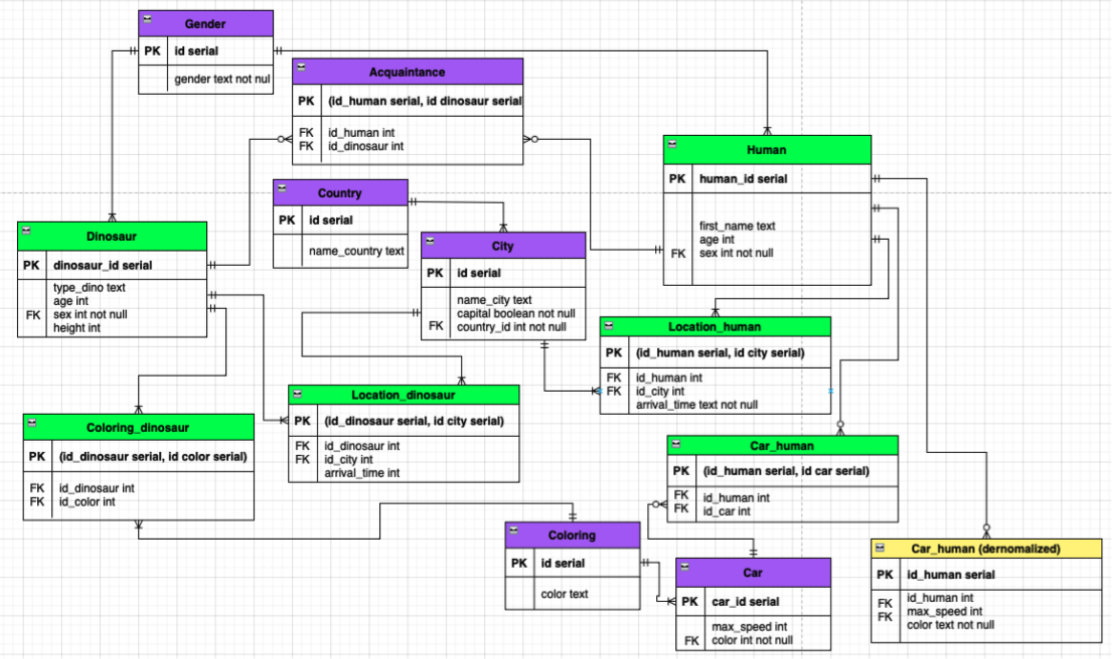
\includegraphics[width=.9\textwidth]{123}